\documentclass [border = .2cm] {standalone}

% Required packages
\usepackage{pgfplots}
\pgfplotsset{compat = newest}
\usetikzlibrary {backgrounds}

\begin{document}
	
	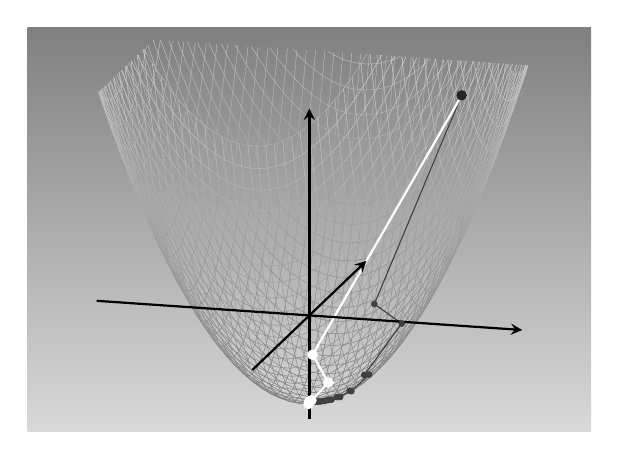
\begin{tikzpicture}		
		[background rectangle/.style=
		{bottom color=white!70!gray!},
		show background rectangle]
		
		\begin{axis}[
			 view = {15}{20},
			 colormap={blackwhite}{gray(0cm)=(0.5); gray(1cm)=(1)},
			 thick,
			 axis lines = center,
			 axis on top,
			 color=black,
			 xmax = 10,
			 xmin = -10,
			 ymax = 3, 
			 ymin = -3, 
			 zmax = 12, 
			 zmin = -6,
			 xticklabels=\empty,
			 yticklabels=\empty,
			 zticklabels=\empty,
			 xtick=false,
			 ytick=false,
			 ztick=false,
			 ]
			
			\addplot3 [
			domain=-10:10,
			domain y = -3:3,
			samples = 50,
			samples y = 50,
			surf,
			mesh,
			ultra thin,
			shader = interp,
			no marks,
			] {0.2 * x^2 + 2 * y^2 - 5};
			
		
		
			\addplot3 [
			color=gray!50!black!,
			thin,
			mark=*,
			mark size=1pt,
			draw=gray!50!black!,			
			] coordinates 
			{
				(5.1, 2.3, 10.78)
				(4.28400000000000, -1.38000000000000, 2.47933120000000)
				(3.59856000000000, 0.828000000000001, -1.03890518528000)
				(3.02279040000000, -0.496800000000000, -2.67892715953357)
				(2.53914393600000, 0.298080000000000, -3.53284624165489)
				(2.13288090624000, -0.178848000000000, -4.02619059375137)
				(1.79161996124160, 0.107308800000000, -4.33498922578125)
				(1.50496076744295, -0.0643852800000001, -4.53872768913016)
				(1.26416704465207, 0.0386311680000001, -4.67739160236105)
				(1.06190031750774, -0.0231787008000000, -4.77339903879384)
				(0.891996266706503, 0.0139072204800000, -4.84048171047338)
				(0.749276864033463, -0.00834433228800002, -4.88757758044218)
				(0.629392565788109, 0.00500659937280001, -4.92072286755158)
				(0.528689755262011, -0.00300395962368001, -4.94407938098936)
				(0.444099394420089, 0.00180237577420801, -4.96054864845828)
				(0.373043491312875, -0.00108142546452480, -4.97216537175575)
				(0.313356532702815, 0.000648855278714882, -4.98036069465615)
				(0.263219487470365, -0.000389313167228929, -4.98614279715369)
				(0.221104369475106, 0.000233587900337358, -4.99022246243319)
				(0.185727670359089, -0.000140152740202415, -4.99310100720702)
				(0.156011243101635, 0.0000840916441214488, -4.99513208426237)
				(0.131049444205373, -0.0000504549864728693, -4.99656520354329)
				(0.110081533132514, 0.0000302729918837216, -4.99757640937974)
				(0.0924684878313114, -0.0000181637951302329, -4.99828991509180)
				(0.0776735297783016, 0.0000108982770781398, -4.99879336431682)
				(0.0652457650137734, -6.53896624688386E-6, -4.99914859794404)
				(0.0548064426115696, 3.92337974813032E-6, -4.99939925073887)
				(0.0460374117937185, -2.35402784887819E-6, -4.99957611133199)
				(0.0386714259067235, 1.41241670932691E-6, -4.99970090415968)
				(0.0324839977616478, -8.47450025596149E-7, -4.99978895797645)
				(0.0272865581197841, 5.08470015357689E-7, -4.99985108874868)
				(0.0229207088206187, -3.05082009214614E-7, -4.99989492822125)
				(0.0192533954093197, 1.83049205528768E-7, -4.99992586135298)
				(0.0161728521438285, -1.09829523317261E-7, -4.99994768777069)
				(0.0135851958008160, 6.58977139903566E-8, -4.99996308849101)
				(0.0114115644726854, -3.95386283942140E-8, -4.99997395523926)
				(0.00958571415705574, 2.37231770365284E-8, -4.99998162281682)
				(0.00805199989192682, -1.42339062219170E-8, -4.99998703305955)
				(0.00676367990921853, 8.54034373315022E-9, -4.99999085052682)
				(0.00568149112374356, -5.12420623989013E-9, -4.99999354413173)
				(0.00477245254394459, 3.07452374393408E-9, -4.99999544473935)
				
			};
		    
			\addplot3 [
			color=white,
			thick,
			mark=*,	
			mark size=1.5pt,		
			draw=white,
			] coordinates 
			{
				(5.1, 2.3, 10.78)
				(1.40000181372460, -1.39999959782613, -0.688001236486907)
				(0.420548264150597, 0.523803523826846, -4.41588756835715)
				(0.127254829139659, -0.182733715958336, -4.92997801979625)
				(0.0385318995324591, 0.0632032462803674, -4.99171375786294)
				(0.0116679060510461, -0.0218380283970381, -4.99901897302514)
				(0.00353319693096165, 0.00754456381439479, -4.99988366241760)
				(0.00106989950621102, -0.00260644449389353, -4.99998618395722)				
			};
		
			\addplot3 [
			color=gray!30!black!,
			mark=*,	
			mark size=1.5pt,	
			] coordinates 
			{
				(5.1, 2.3, 10.78)
				
			};
			
				
		\end{axis}
		
	\end{tikzpicture}
	
\end{document}